\documentclass[12pt, a4paper]{article}
\usepackage[utf8]{inputenc}
\usepackage{graphicx}
\usepackage{gensymb}
\usepackage{amsmath}
\usepackage{float}
\usepackage{subcaption}
\usepackage{caption}


\title{Fast Fourier transform and correlation functions}
\author{Miha Pompe}
\date{November 2021}

\begin{document}
\begin{titlepage}
	\centering
 	
\includegraphics[width=0.45\textwidth]{logo_fmf_uni-lj_sl_veliki.png}\par\vspace{1cm}

	\vspace{1cm}

	\vspace{1.5cm}
	{\huge\bfseries Fast Fourier transform and correlation functions\par}
	\vspace{2cm}
	{\Large Miha Pompe 28191072\par}
	\vfill

	\vfill

% Bottom of the page
	{\large November 2021\par}
\end{titlepage}
% \maketitle
\thispagestyle{empty}
\clearpage
\pagenumbering{arabic}
\newpage


\section{Introduction}
Fast Fourier transform (FFT) is a very useful tool for analyzing different kinds of signals. Its benefits are high speed and low memory consumption. These two properties will allow us to analyze longer signal compared to normal discrete Fourier transform (DFT). With a clever implementation we can reduce the time complexity to $N log_2N$, down from $N^2$. Comparison of these two implementations was presented in the previous report. We will use Fourier transforms to help us calculate correlation functions, which are defined as:

\begin{equation*}
  \phi_{gh}(\tau)=\frac{1}{T}\int\limits_0^{T} g(t+\tau)\,h(t)\dd t \>,  
\end{equation*}
or for discrete values
\begin{equation*}
  \phi_{gh}(n)= \frac{1}{N}\sum_{k=0}^{N-1} g_{k+n}\, h_k \>.
\end{equation*}

With the help of Fourier transforms we can convert convolution to multiplication. Let $F = \mathcal{F}(f)$ and $G = \mathcal{F}(g)$, then correlation function is given as:
\begin{equation*}
  \phi_{gh}(n) = \frac{1}{N-n}\mathcal{F}^{-1} \left[ G \cdot (H)^\ast \right]
\end{equation*}
To calculate the autocorrelation function we use the equation above, where $g = h$.

\section{Performance analysis}
The implemented code for FFT and correlation calculation mainly uses built in functions from {\sc numpy} and {\sc scipy}. Functions used are {\sc np.fft.fft} (FFT Numpy), {\sc scipy.fft.fft} (FFT Scipy), and {\sc numpy.signal.fftconvolve} (Autocor. Numpy). The accuracy of those functions was already tested in the previous report. Another method (Autocor. FFT) was used to calculate the correlation function which follows the formula from Introduction.

Computation time of all the used methods is presented in Figure 1. The fastest method is the manually implemented correlation, because we only have to multiply two Fourier transforms. If we included FFT calculation the method would be similar to FFT Numpy and Autocor. Numpy. Second and third are FFT Scipy and FFT Numpy respectively. The slowest one is correlation done using a Numpy function. Based on documentation we know that the algorithm of this method is similar to the one I implemented.

\begin{figure}[hbtp]
  \begin{center}
  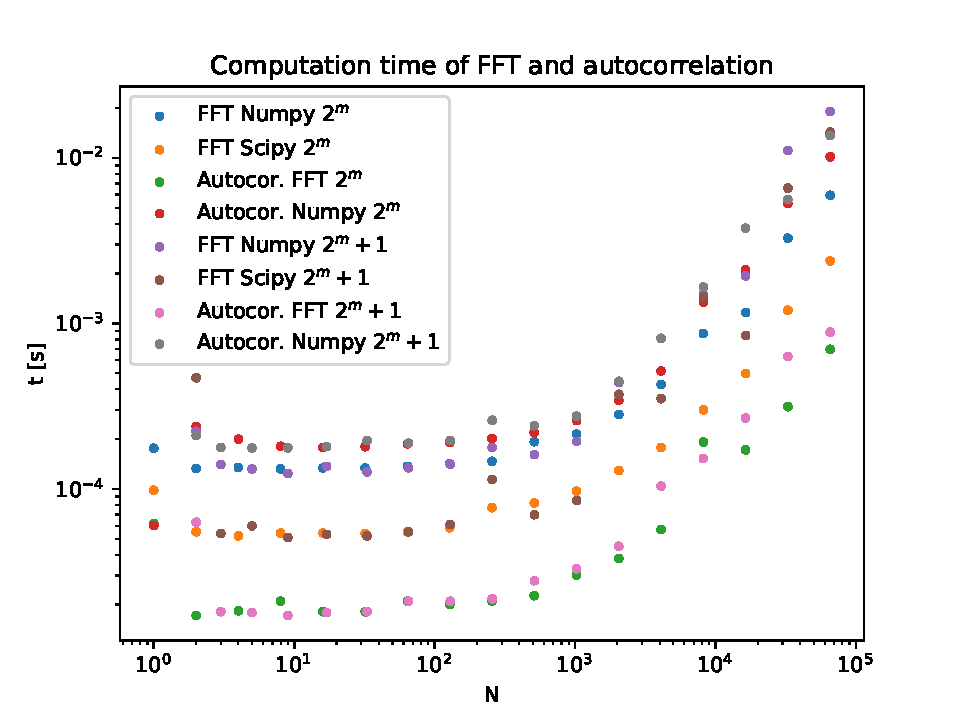
\includegraphics[width=11cm]{graphs/time_FFT_5.pdf}
  \end{center}
  \vspace*{-7mm}
  \caption{Computation time of different FFT and autocorrelation methods, evaluated at different sizes of input signals.}
\end{figure}

With small input signals ($N < 100$) the calculation times is almost constant. With larger $N$ the curve follows $Nlog_2N$ (straight line on log-log scale). 

I also compared how the number of elements used for calculation affects the performance. Two different types of sizes were used; $N = 2^m$ and $N = 2^m+1$ where $m \in \{0, 1, 2, \dots\}$. Due to the recursive implementation of FFT, signals with length $N = 2^m$, should be computed faster. This is exactly what we see on Figure 1 in the majority of cases.

\begin{figure}[hbtp]
  \centering
  \begin{subfigure}{\textwidth}
    \centering
    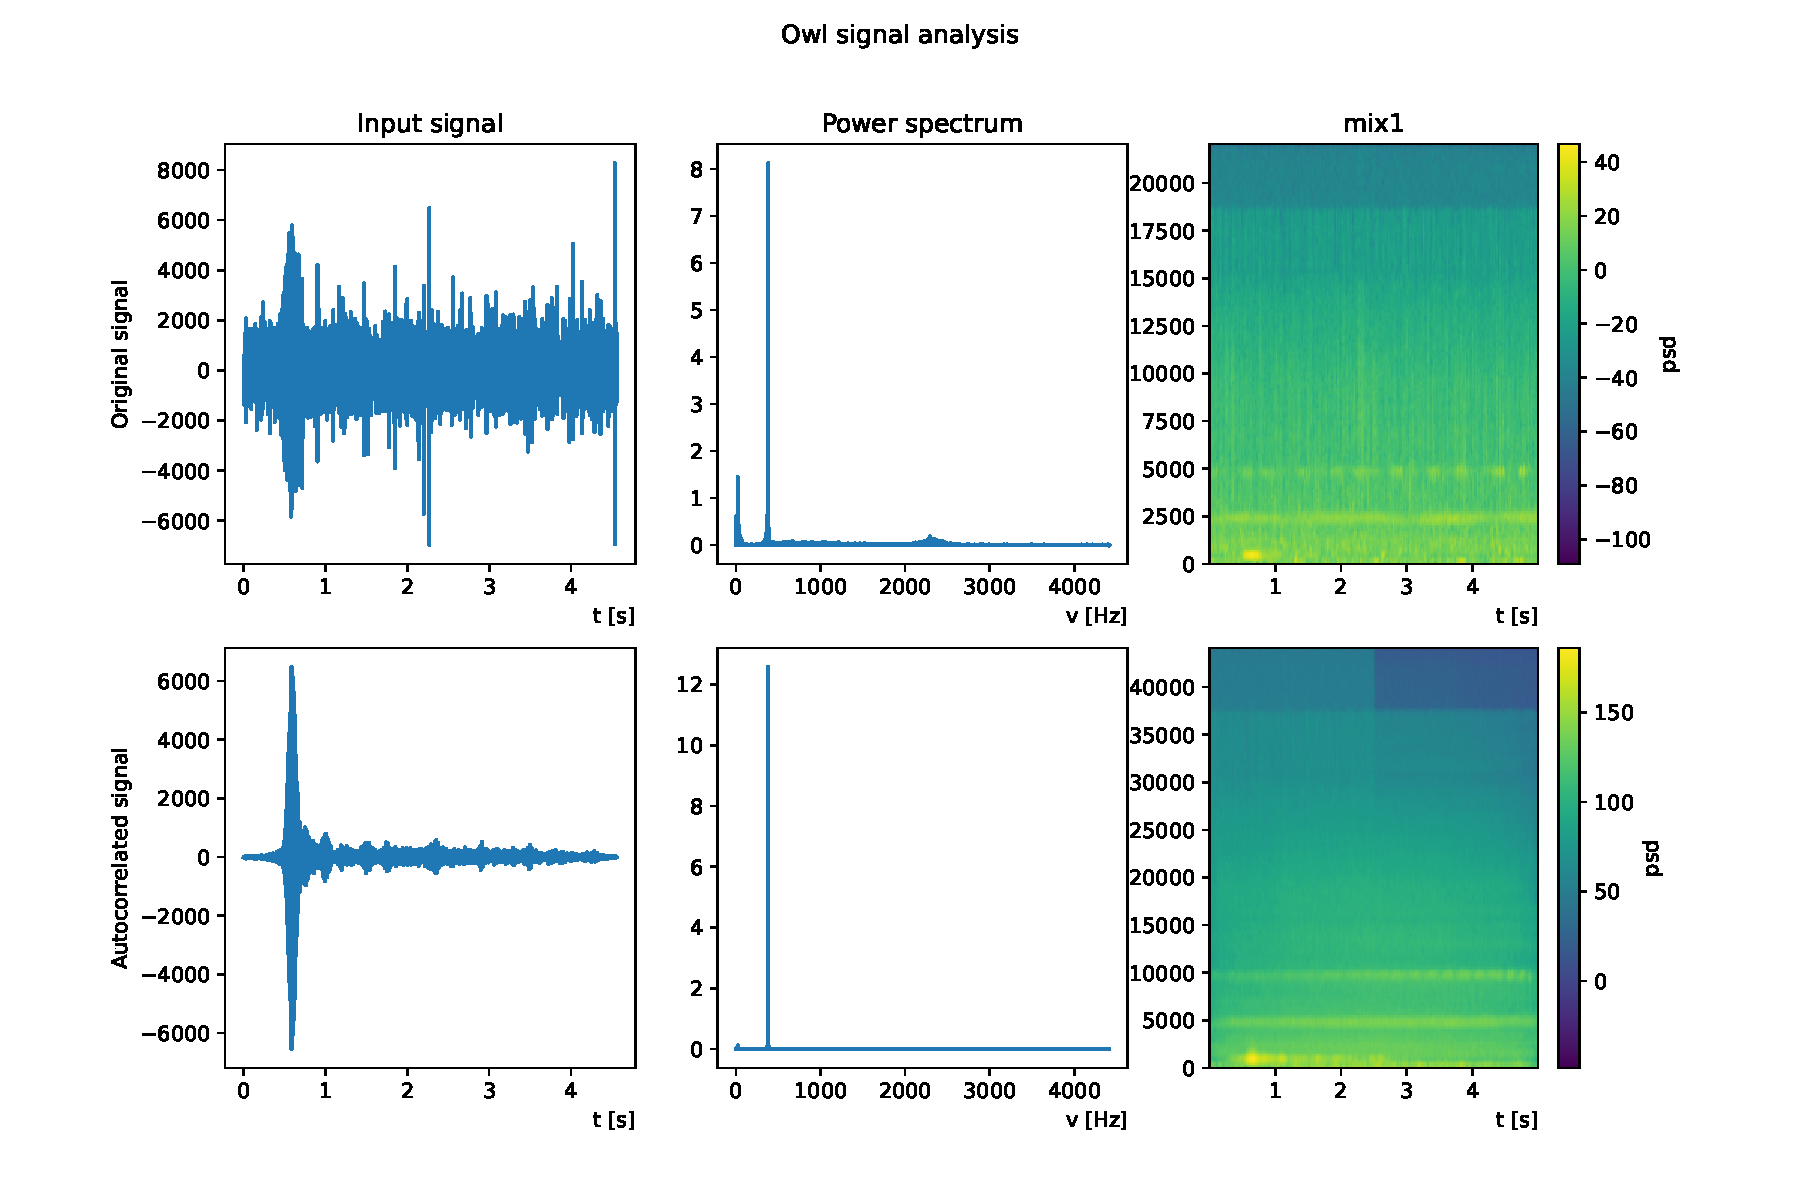
\includegraphics[width=\linewidth]{graphs/spectrogram4.pdf}
    \caption{Owl audio signal analysis. The first row contains the original signal and the second one the autocorrected signal.}
    \label{fig:sub1}
  \end{subfigure} 
  
  \begin{subfigure}{\textwidth}
    \centering
    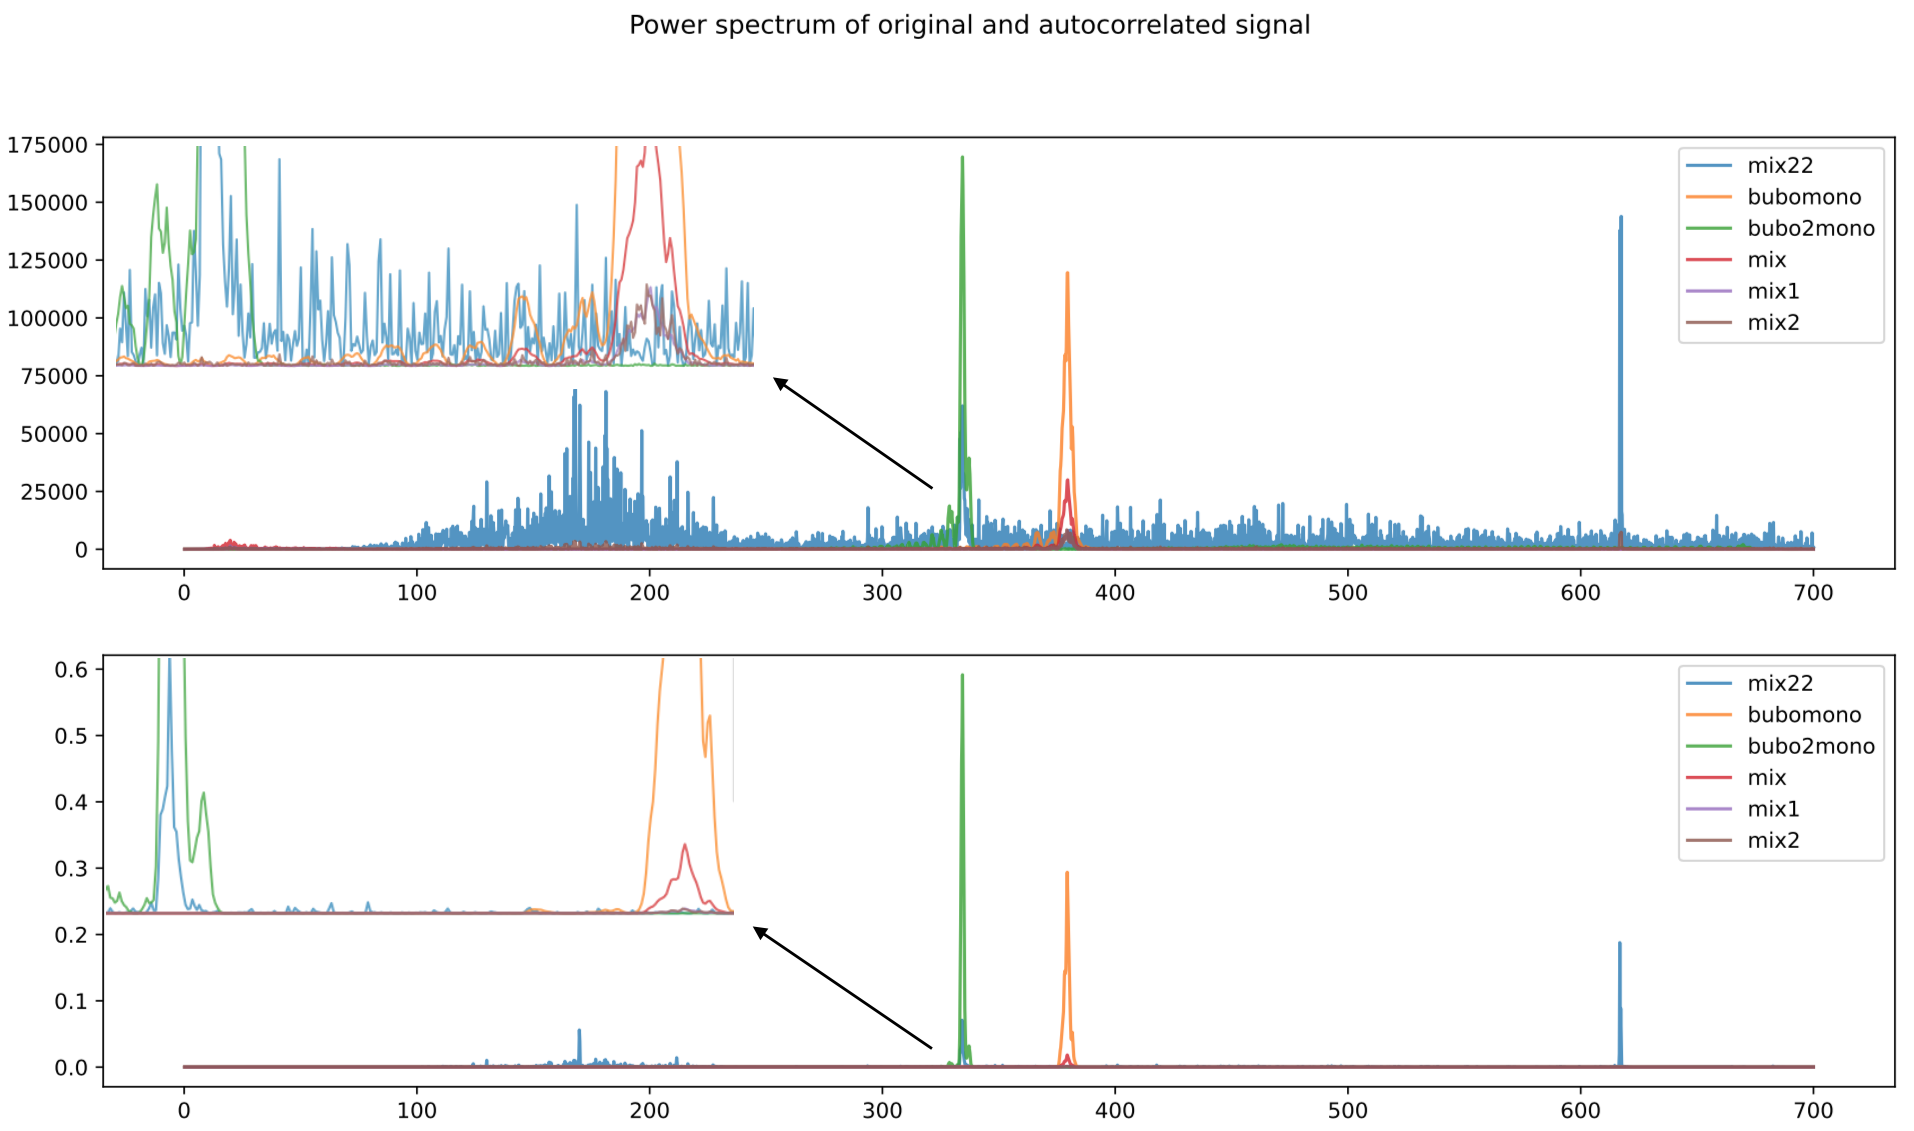
\includegraphics[width=\linewidth]{graphs/spectrum_zoom_photo.png}
    \caption{Levyjev pobeg}
    \label{fig:sub2}
  \end{subfigure} 
  \caption{Power spectrum of original and autocorrelated signals of all recordings. In the upper left corner is a closeup of the central part.}
  \label{fig:test}
\end{figure}


\section{Owl sound analysis}

Using methods presented above we will analyze sound recordings of owls, bubo and bubo2. Those recordings contain either clean sound or sound masked with noise from the surroundings. Let's first look at the workflow for signal analysis. The first row of Figure 2a shows the analysis of the original signal, in this case we are looking at mix1.waw. What can be observed from the first graph is that there is a substantial amount of noise in this recording, which can also be seen in the power spectrum (high and low frequency noise). The spectrogram shows the power spectrum density (psd) as a function of time and frequency. At around $t = 0.8s$ we can see a short peak corresponding to the owl sound, whereas everything else is noise. To improve the clarity of the signal we can autocorrelate it. This is shown in the second row of Figure 2b. We immediately notice considerably less noise and a very pronounced owl sound. Looking at the power spectrum a similar conclusion can be made. If we compare the spectrogram of the original and autocorrelated signal we can see that the high frequency area is smoother.

Frequency analysis can also help us determine which owl can be heard in each recording. Figure 2b shows the power spectrum of the original and autocorrelated signals. Based on matching peaks we can come to the following conclusions:

\begin{center}
  \begin{tabular}{ c c }
   Recording & Owl \\ 
   \hline
   mix & bubo \\
   mix 1 & bubo \\ 
   mix 2 & bubo \\
   mix 22 & bubo2
  \end{tabular}
\end{center}

Most peaks are observed more easily on the autocorrelated graph. On Figure 2b lines mix1 and mix2 should be scaled for easier observation. Another approach to determining owls is to correlate the clean sound (bubomono or bubo2mono) with every recording. 

\section{Lidar data analysis}
For the extra part I decided to analyze the signal of a very simple Lidar setup. My goal was to see if I could get any information about the distance using simple basic electronics. The setup consists of a laser diode that is flashing with frequency $\nu_f = 50 Hz$, $t_0 = 20 ms$. The light then reflected of a mirror placed at $1.5 m$ or $15 m$. The reflected light is measured using a photoresistor, a voltage divider and a microprocessor. The sampling frequency of the circuit is $\nu_s = 484 Hz$, $t_s = 2.06 ms$. Signal analysis was done offline. The whole setup can be see on Figure 4.

\begin{figure}[hbtp]
  \begin{center}
  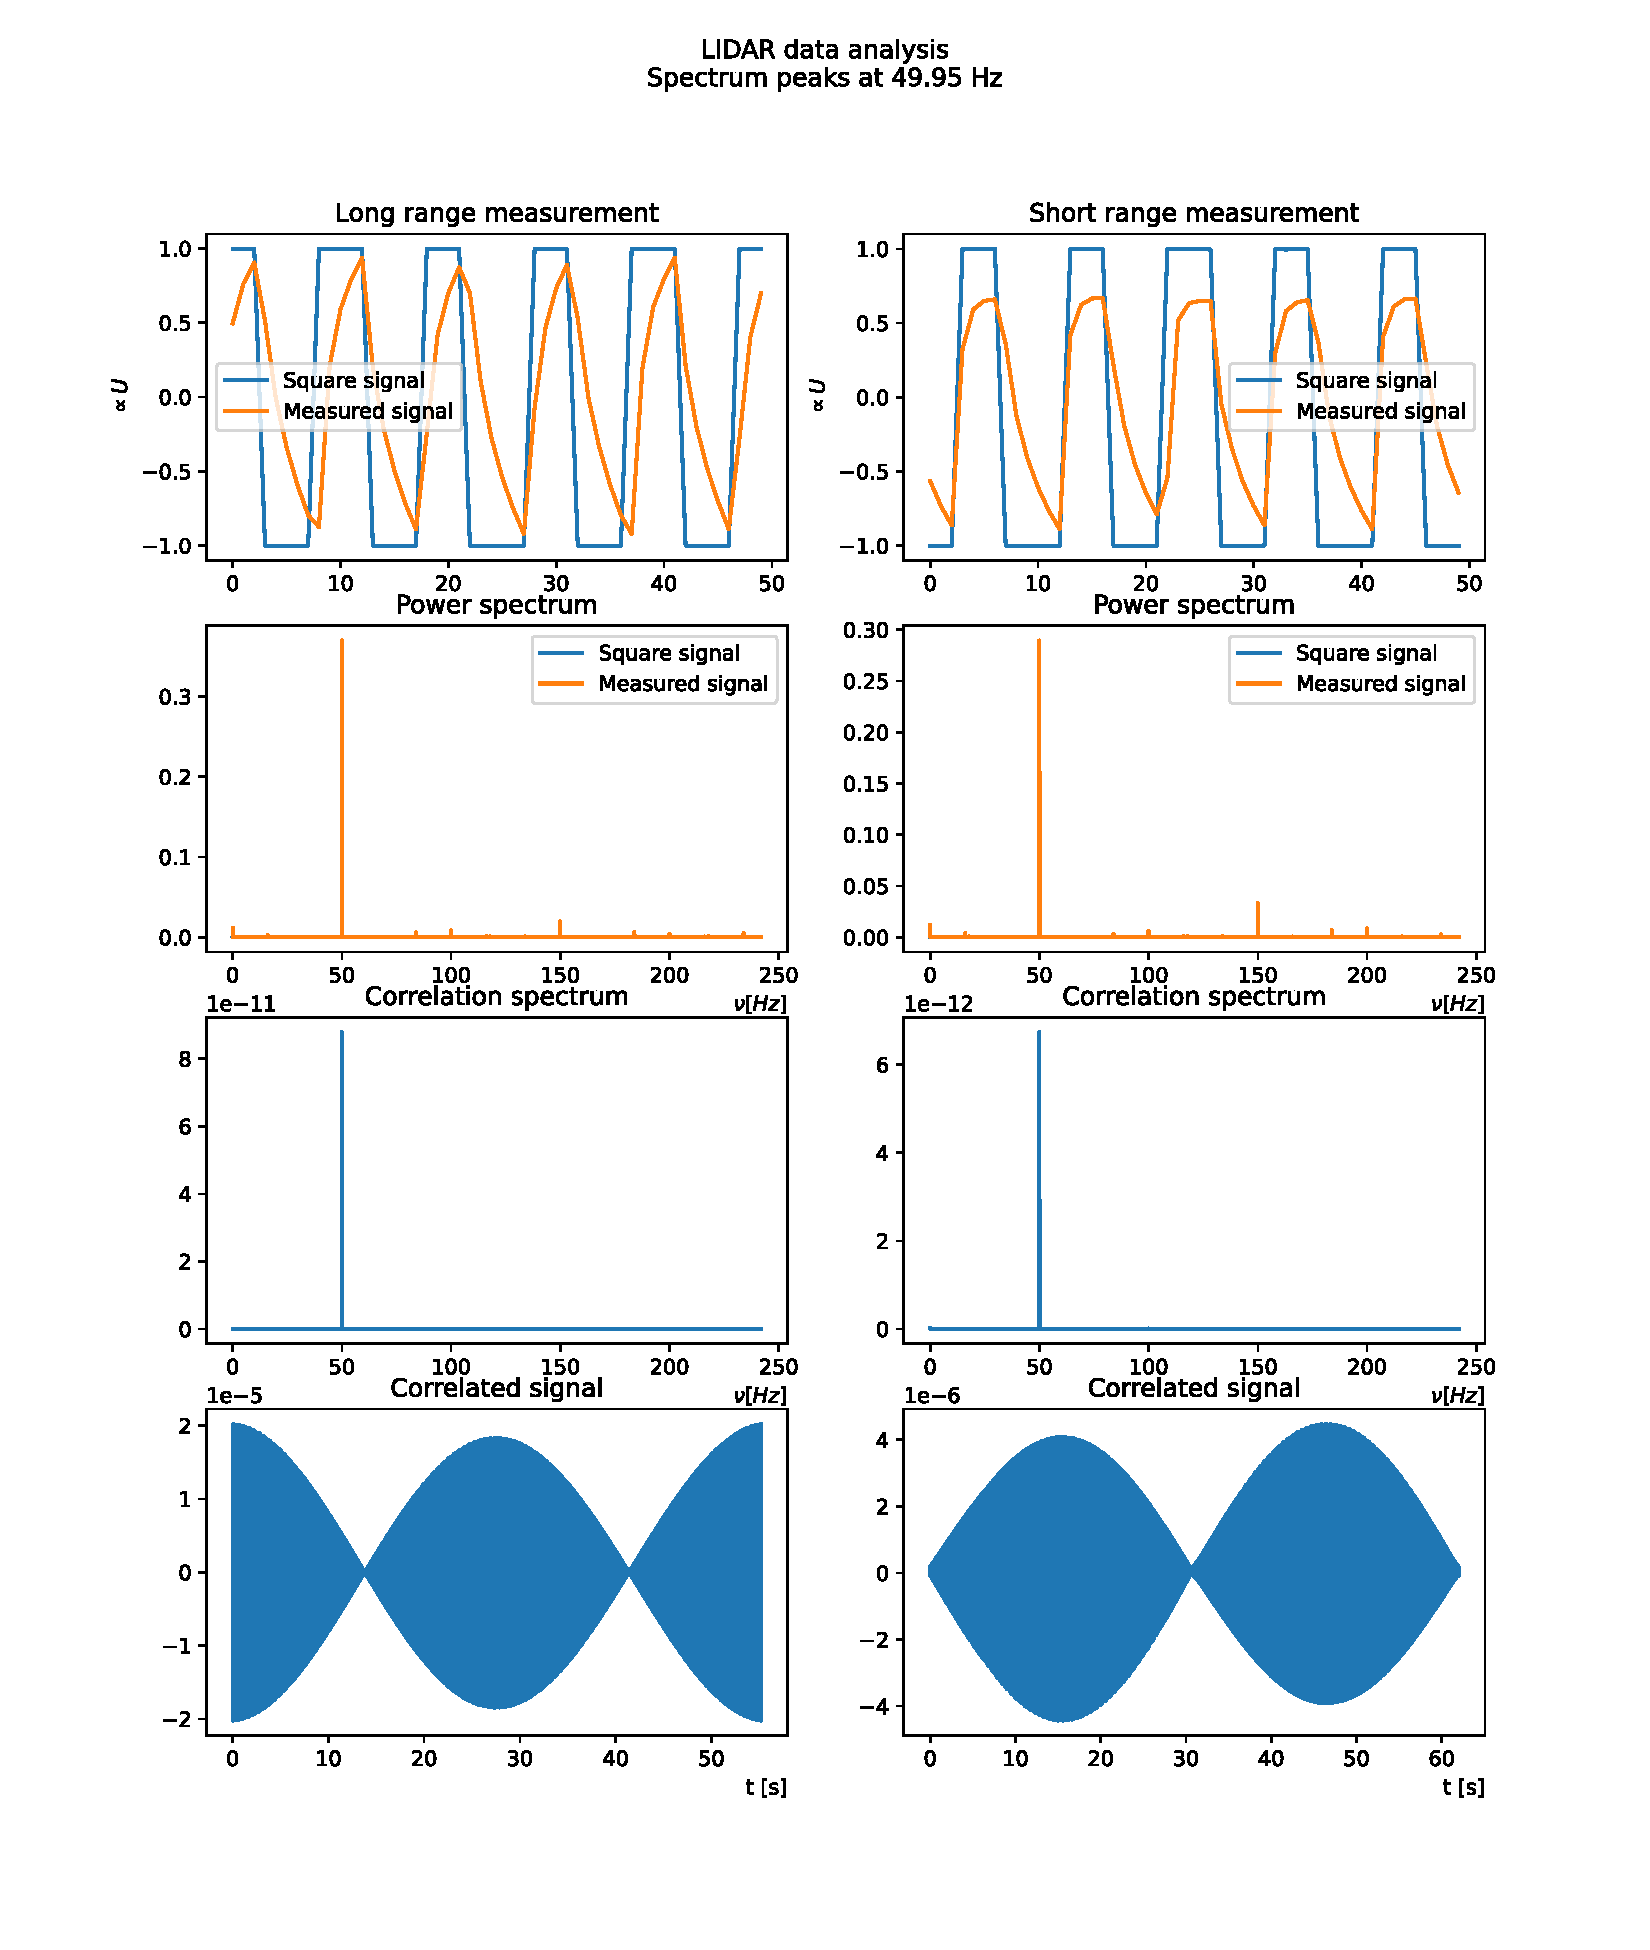
\includegraphics[width=\linewidth]{graphs/lidar.pdf}
  \end{center}
  %\vspace*{-7mm}
  \caption{}
\end{figure}

I performed two experiments with this setup; long and short range observations. They can be seen in the left and right columns in Figure 3. The first two graphs show outbound and incoming signals. The difference in shape comes from the characteristics of the laser. What can be also seen is that pulses are not of the same width, even though they should be, which is the result of clocks not being synced on both devices (generator and analyzer). Looking at the power spectrum we can mainly see the flashing frequency $\nu_f$ and followed by its harmonics. If we correlate the two signals we only see the flashing frequency in the power spectrum. Besides this high frequency we can also see a component with $t_0 \approx 60 s$ which matches with the length of the measurement. In conclusion we were not able to produce any distance data.

\begin{figure}[hbtp]
  \begin{center}
  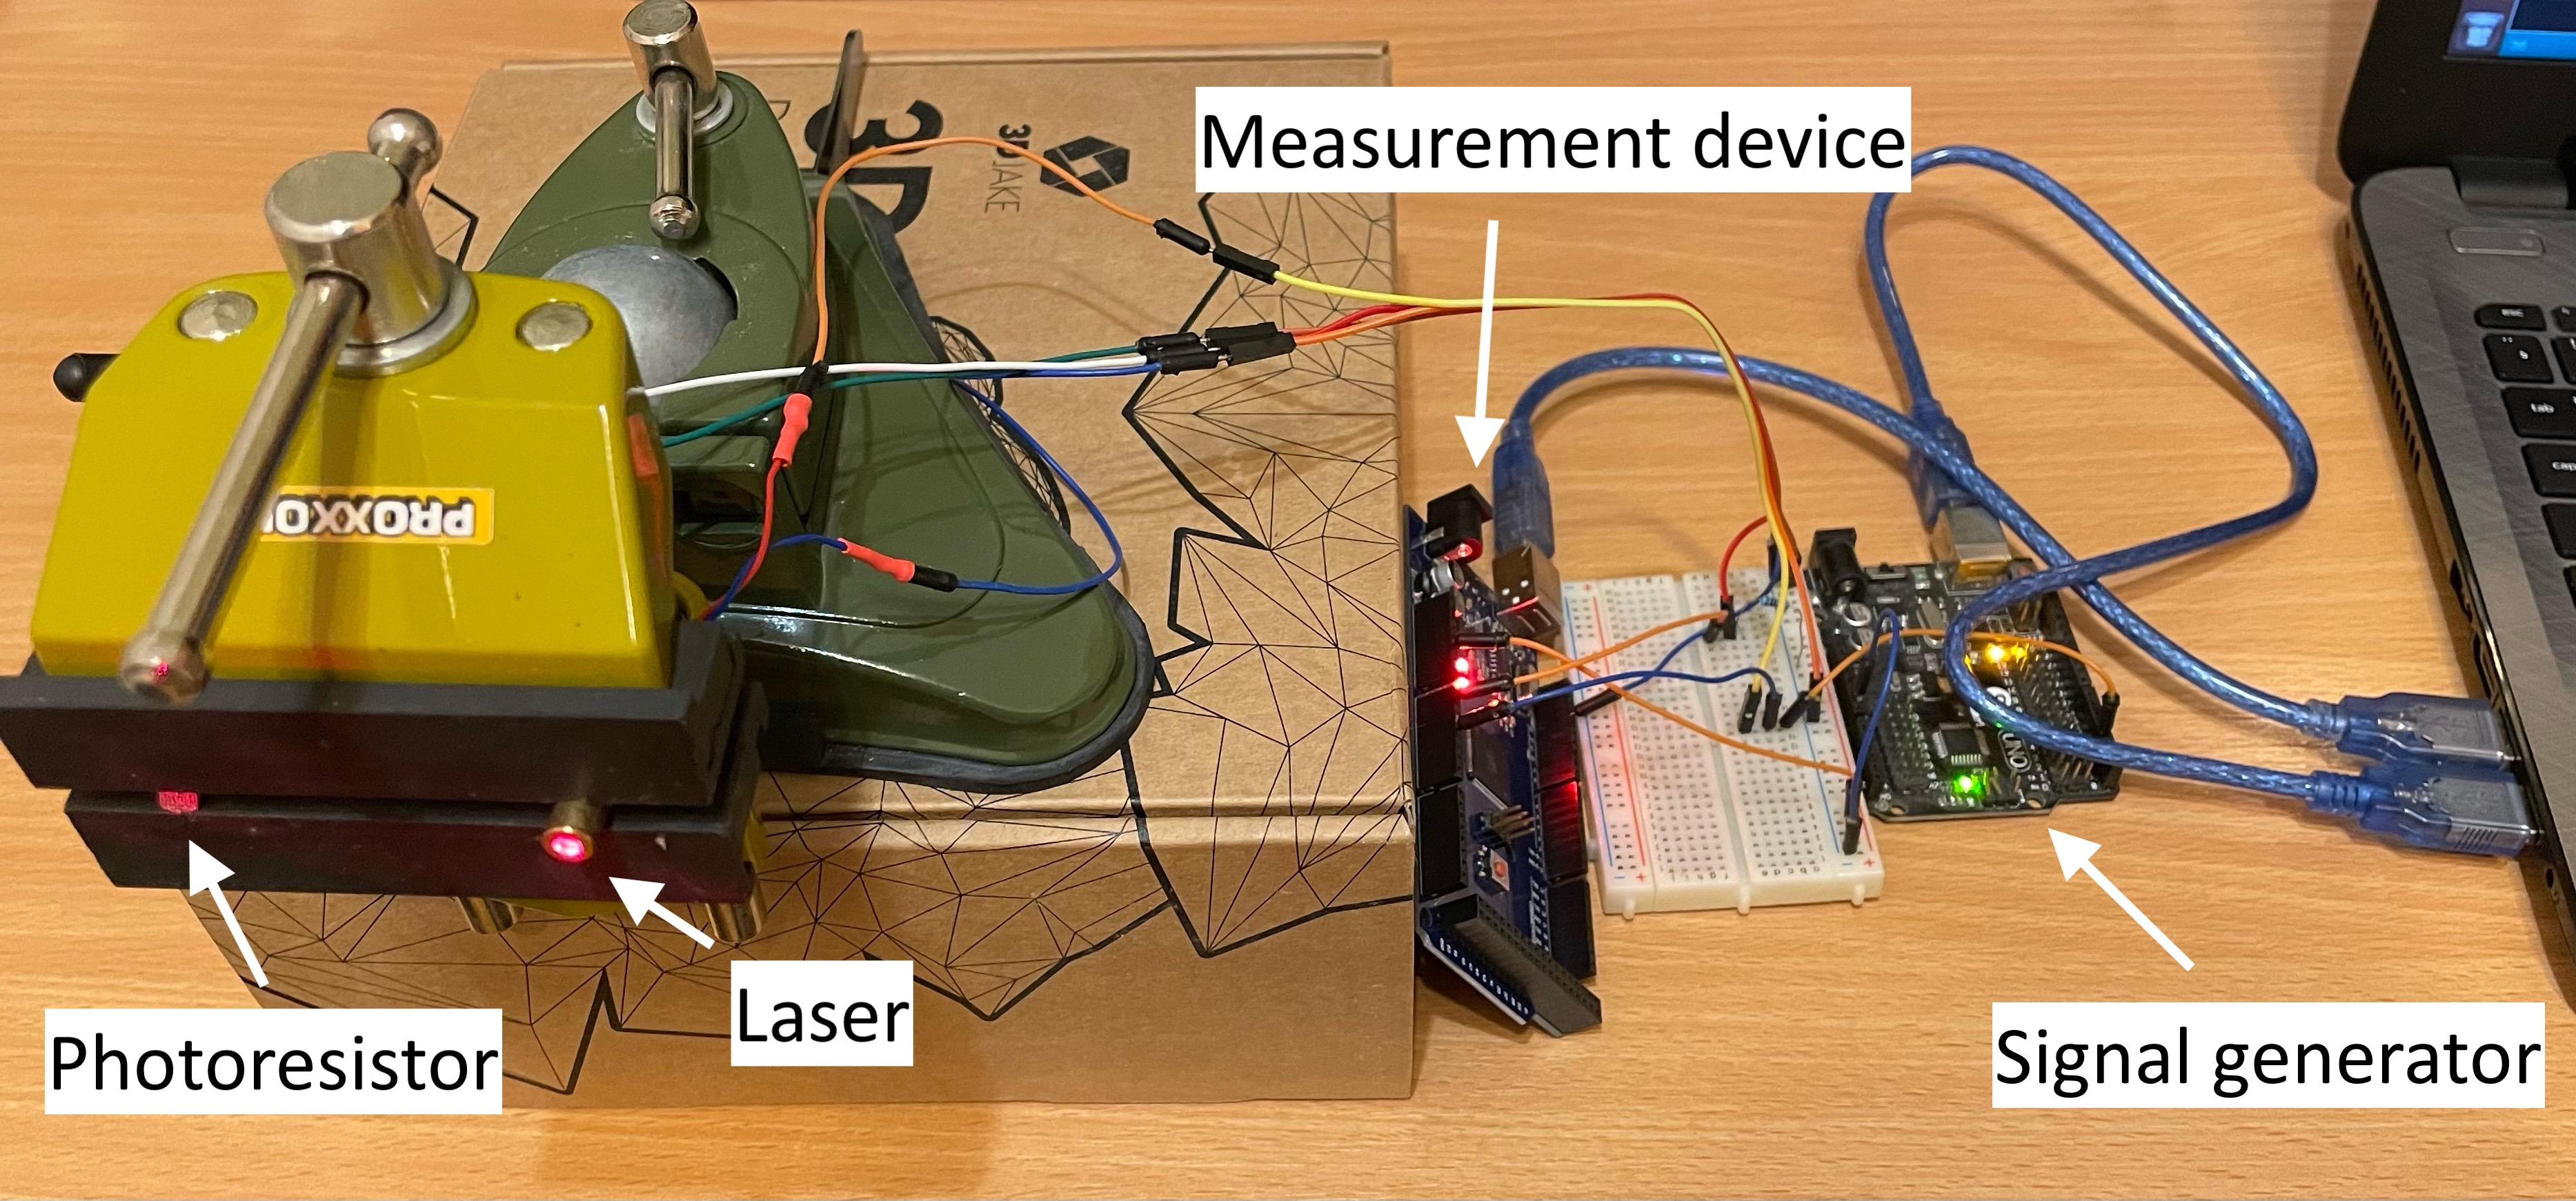
\includegraphics[width=\linewidth]{graphs/IMG_6511.jpeg}
  \end{center}
  %\vspace*{-7mm}
  \caption{Lidar setup}
\end{figure}

The issue in the setup is low sampling frequency and high speed of light. A quick calculation shows that we would need to measure distances of a few hundred kilometers in order to see a delay. In practice this is solved using higher sampling frequencies and by using analog electronics to calculate the phase difference.

A more viable method that could be performed at home is to use sound instead of light. We can exploit the high sample rate of sound recording, which can go from $44.1 kHz$ to $96 kHz$ (for Macs built in microphones). This would allow us to measure distances with resolution of roughly $1 cm$. 


\section{Conclusion}
The aim of this report was to examine different signals, by using fast Fourier transform and correlation functions. The implemented version uses fast and accurate methods to calculate both FFT and correlation function. We successfully determined which owl is in which recording and showed that we cannot build a Lidar using only simple electronics components.

\end{document}

